\documentclass{standalone}
\usepackage[dvipsnames]{xcolor}
\usepackage{pgfplots}
\pgfplotsset{
  compat=1.18, 
  trig format=rad, 
  ticklabel style = {font=\tiny},
  axis equal image,
}
\usepackage{subfiles}

\begin{document}
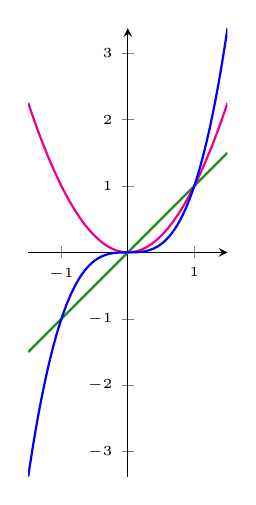
\begin{tikzpicture}
  \begin{axis}[
    axis x line={middle},
    axis y line={middle},
    ytick={-3,-2,-1,0,1,2,3},
    xtick={-1,0,1},
    % xticklabels={\(-2\pi\),,\(-\pi\),,,,\(\pi\),,\(2\pi\)},
    domain={-3/2}:{3/2}
    ]

    % \addplot[thick, smooth, samples=1000, domain=-1:1] {asin(x)/180*pi};
    \addplot[ForestGreen, thick, smooth, samples=1000] {x};
    \addplot[magenta, thick, smooth, samples=1000] {x^2};
    \addplot[Blue, thick, smooth, samples=1000] {x^3};
  \end{axis}
\end{tikzpicture}
\end{document}
